\documentclass[11pt]{report}
\usepackage{color}
\usepackage{graphicx}
\DeclareGraphicsExtensions{.pdf,.png,.jpg}
\usepackage[margin=1.2in]{geometry}
\usepackage{rotating}
\usepackage[utf8]{inputenc}
\usepackage{multirow}
\usepackage[table,xcdraw]{xcolor}
\usepackage{indentfirst}
\usepackage{graphicx}
\usepackage{booktabs}
\usepackage{tabularx} 
\usepackage{tabulary}
\usepackage{cutwin}
\usepackage{caption}
\usepackage{lipsum}
\usepackage{wrapfig}
\usepackage{color}
\usepackage{eurosym}
\usepackage{subcaption}
\usepackage{amsmath}
\usepackage{titlesec}
\usepackage{enumerate}
\usepackage{listings}
\usepackage{cite}
\usepackage{float}

\definecolor{ritagreen}{rgb}{0.0, 0.71, 0.0}
\definecolor{mygreen}{rgb}{0,0.6,0}
\definecolor{mygray}{rgb}{0.5,0.5,0.5}
\definecolor{mymauve}{rgb}{0.58,0,0.82}

\lstnewenvironment{EL}{
\lstset{
	emph={interface, compile, language, component, properties, services, references, subcomponents, bind, to, annotation, int, string, float, promote, service, reference, is, import, elaboration, property, value, element}, 
	emphstyle=\color{purple}\textbf,
	basicstyle=\ttfamily,
	tabsize=1,
	frame=single,
	breaklines=true,
	morecomment=[s][\color{blue}]{"}{"},
	commentstyle=\color{ritagreen},
	morecomment=[l]{//},
	morecomment=[s]{/*}{*/},
	numbers=left,
	stepnumber=1,    
	firstnumber=1,
	numberfirstline=true,
	numberstyle=\tiny\color{mygray}
}}{}

\lstnewenvironment{Cpp}{
	\lstset{
		emph={if, endif, true}, 
		emphstyle=\color{purple}\textbf,
		basicstyle=\ttfamily,
		tabsize=1,
		frame=single,
		breaklines=true,
		morecomment=[s][\color{blue}]{"}{"},
		commentstyle=\color{ritagreen},
		morecomment=[l]{//},
		morecomment=[s]{/*}{*/},
		numbers=left,
		stepnumber=1,    
		firstnumber=1,
		numberfirstline=true,
		numberstyle=\tiny\color{mygray}
	}
}{}

\lstnewenvironment{ARM}{
	\lstset{
		emph={LDRH, ADDW, STRH, LDRB}, 
		emphstyle=\textbf,
		basicstyle=\ttfamily,
		tabsize=1,
		frame=single,
		breaklines=true,
		commentstyle=\color{ritagreen},
		morecomment=[l]{;},
		numbers=left,
		stepnumber=1,    
		firstnumber=1,
		numberfirstline=true,
		numberstyle=\tiny\color{mygray}
	}
}{}


\lstset{
	basicstyle=\ttfamily,
	tabsize=1,
	frame=single,
	breaklines=true,
	morecomment=[s][\color{blue}]{"}{"},
	commentstyle=\color{ritagreen},
	morecomment=[l]{//},
	morecomment=[s]{/*}{*/},
	numbers=left,
	stepnumber=1,    
	firstnumber=1,
	numberfirstline=true,
	numberstyle=\tiny\color{mygray}
}


\newenvironment{abbreviations}{\begin{list}{}{\renewcommand{\makelabel}{\abbrlabel}}}{\end{list}}
\newcommand{\abbrlabel}[1]{\makebox[3cm][l]{\textbf{#1}\ \dotfill}}

\titleclass{\subsubsubsection}{straight}[\subsection]
\newcounter{subsubsubsection}[subsubsection]
\renewcommand\thesubsubsubsection{\thesubsubsection.\arabic{subsubsubsection}}
\renewcommand\theparagraph{\thesubsubsubsection.\arabic{paragraph}} % optional; useful if paragraphs are to be numbered
\titleformat{\subsubsubsection}
{\normalfont\normalsize\bfseries}{\thesubsubsubsection}{1em}{}
\titlespacing*{\subsubsubsection}
{0pt}{3.25ex plus 1ex minus .2ex}{1.5ex plus .2ex}
\makeatletter
\renewcommand\paragraph{\@startsection{paragraph}{5}{\z@}%
	{3.25ex \@plus1ex \@minus.2ex}%
	{-1em}%
	{\normalfont\normalsize\bfseries}}
\renewcommand\subparagraph{\@startsection{subparagraph}{6}{\parindent}%
	{3.25ex \@plus1ex \@minus .2ex}%
	{-1em}%
	{\normalfont\normalsize\bfseries}}
\def\toclevel@subsubsubsection{4}
\def\toclevel@paragraph{5}
\def\toclevel@paragraph{6}
\def\l@subsubsubsection{\@dottedtocline{4}{7em}{4em}}
\def\l@paragraph{\@dottedtocline{5}{10em}{5em}}
\def\l@subparagraph{\@dottedtocline{6}{14em}{6em}}
\makeatother
\setcounter{secnumdepth}{4}
\setcounter{tocdepth}{4}


\begin{document}
	
\begin{titlepage}
	\centering
	\vspace*{0.5 cm}
	
\includegraphics[scale = 0.75]{Images/umee}\\[1.0 cm]
	\textsc{\LARGE University of Minho}\\[2.0 cm]
	\textsc{\Large Project II}\\[0.5 cm]		
	\textsc{\large Integrated Master in Electronics and Computer Engineering}\\[0.5 cm]				% Course Name
	\rule{\linewidth}{0.2 mm} \\[0.4 cm]
		{ \huge \bfseries Final Report} \\
        { \huge \bfseries Modeling for Dynamic Binary Translation \\
			\LARGE \bfseries Code Generation}
		
	\rule{\linewidth}{0.2 mm} \\[1.5 cm]
		
		\begin{minipage}{0.4\textwidth}
			\begin{flushleft} \large
				\emph{Authors:}\\
				Ana Rita Fernandes Martins\\
				David Miguel Parente Almeida
			\end{flushleft}
		\end{minipage}~
		\begin{minipage}{0.4\textwidth}
			\begin{flushright} \large
				\emph{Advisors:} \\
				Adriano Tavares\\
				Filipe Salgado
			\end{flushright}
		\end{minipage}\\[2 cm]
		
	{\large Guimarães, \today }\\[2 cm]
		
	\vfill
	
\pagenumbering{gobble}
\end{titlepage}
	
\newpage

%-------------------------------------------
\pagenumbering{roman}  
\tableofcontents
\newpage
%-------------------------------------------	
\listoffigures
\newpage
%-------------------------------------------	
\listoftables
\newpage
%-------------------------------------------
\section*{Abbreviations}
%please put in alfabetical order
\begin{abbreviations} 
	\item[CC] Condition Codes
	\item[CPU] Control Processing Unit
	\item[DBT] Dynamic Binary Translation
	\item[DSL] Domain Specific Language
	\item[EL] Elaboration Language
	\item[ISA] Instruction Set Architecture
	\item[LR] Link Register
	\item[PC] Program Counter
	\item[SCA] Service Component Architecture
	\item[SFR] Special Function Registers
	\item[SP] Stack Pointer
	\item[XML] eXtensible Markup Language
\end{abbreviations}
\newpage
%-------------------------------------------	
\pagenumbering{arabic}
%START ABSTRACT CHAPTER
\chapter{Abstract}

\par Creating a model for an embedded system provides a time-saving and cost-effective approach to the development of dynamic systems, based on a single model maintained in a tightly integrated software. 
\par Using modern modeling software tools it is possible to design and perform initial validation. It is possible to reduce the risk of errors and shorten development time by performing verification and validation testing throughout the development. Errors and overhead can also be reduced through the use of automatic code generation techniques\cite{j.h.foleissa.l.t.d'amatoa.f.dasilva2012}.
\par With these advantages in mind, it was developed a Domain Specific Language in the context of the master's degree in Embedded Systems, the Elaboration Language, to easily create models of a given reference architecture. In this project, it is used the reference architecture of a dynamic binary translator to prove the efficiency of the tool.


%END ABSTRACT CHAPTER
%-------------------------------------------
%START ANALYSIS CHAPTER
\chapter{Analysis}

	\section{Motivation}
	
	\par The main motivation for this project is the use of the modeling framework developed with the other groups in a real case. Modeling is a technique very valuable for any engineer, so using the Elaboration Language and respective code generation for this purpose was very interesting. 
	\par In the other side, the dynamic binary translation is very challenging and the group had a big interest to see how this technique works.

	\section{Objectives}
	
	\par The objectives of this work are:
	\begin{itemize}
		\item Identifying the modules of the reference architecture;
		\item Modeling the implementation of a dynamic binary translation;
		\item Successful generation of the final source files;
		\item Create parameterized code;
		\item Understand the concepts behind modeling.
	\end{itemize}

	\section{Problem Statement}
	
	\par Modeling is used in order to automate the configuration, generation and validation of the final system. To create a model it is necessary a specialized framework, and the one used in this project was developed together with all the groups in the context of the major in Embedded Systems, consisting on a Domain Specific Language (DSL) which purpose is to model reference architectures and execute its respective code generation. 
	\par In this particular case, the modeling framework is used with the objective to model a DBT, in which the source code follows a 8051 Instruction Set Architecture (ISA) and the translated code is generated for a ARMv7-M ISA.  The reference architecture was agreed by all the groups that are into this project, and this group focus is on the characterization, modeling and code generation for the target architecture and code optimization. The image \ref{fig:compiler-sequence} shows the catalog that is being develop for the Elaboration Language.
	
	\begin{figure} [H]
		\centering
		\includegraphics[width=0.7\linewidth]{Images/DSL_use_cases}
		\caption{Compilation phases.}
		\label{fig:compiler-sequence}
	\end{figure}

	\section{Modeling Languages}
	\par A modeling language is any artificial language that can be used to express information or knowledge of systems in a structure that is defined by a consistent set of rules. The rules are used for interpretation of the meaning of the components in the structure. They can be graphical or textual.
	\par Graphical modeling languages use a diagram technique with named symbols that represent concepts and lines that connect the symbols and represent relationships and various other graphical notation to represent constraints.
	\par Textual modeling languages may use standardized keywords accompanied by parameters or natural language terms and phrases to make computer-interpretable expressions.
	\par Not all modeling languages are executable, and for those that are, the use of them does not necessarily mean that programmers are no longer required. On the contrary, executable modeling languages are intended to amplify the productivity of skilled programmers, so that they can address more challenging problems, such as parallel computing and distributed systems\cite{wikipedia}.
		
		\subsection{Domain Specific Languages}
		
		\par DSL are programming languages, commonly with a small set of expressions, with the objective of abstracting and simplifying the code written for a specific case. So, these languages are useful just when used in that specific situation. Tough they may look limited at a first glance, they may have all the necessary resources to write code for a determined domain.
		\par The usage of these languages should be simple enough in a way that the model is be the biggest effort done. A model should also be translated into code very intuitively by the user. It is important to note that the user is not always a designer: a DSL should be clear at the point that someone who is not used to programming languages could create its script without a lot of effort. The simplicity is pointed as an advantage, but there are disadvantages too: creating a framework like this requires a lot of technical skills and knowledge, and the development is very time consuming.
		\par To write a DSL it is necessary to write a set of grammatic rules that check the desired operation of the language. Then, it is necessary to gather all the requirements to avoid subjectiveness and to specify all the semantics. It is also important to implement software capable of validate the code, type checking and scoping.
		%\par To write a DSL it is necessary to gather all the requirements to avoid subjectiveness and to specify all the semantics. Then, it is written a set of grammatic rules that check the desired operation of the language. It is also important to implement software capable of validate the code, type checking and scoping.
		\par After writing all of this software, it is necessary to implement engines that provide code generation. If the code generation is done nicely, the resulting behavioral model is correct.
		
		\subsection{Service Component Architecture}
		
		\par Service Component Architecture (SCA) is a programming model for abstracting functions as components and using them as building blocks to assemble solutions. A component offers services and depends on functions that are called references.
		\par SCA provides a declarative way to describe how the services interact with one another. Since service interaction is declarative, solution developers remain focus on logic and therefore development cycle is simplified and shortened. This also promotes the development of reusable services that can be used in different contexts. For example, a shopping cart service can be used in a retail application or a travel application without changing. Services can interact with one another synchronously or asynchronously and can be implemented in any technology.
		\par SCA also brings flexibility to deployment. A solution assembled with SCA is deployed as a unit and can be distributed over one or more nodes in the network and can be reconfigured without programming changes \cite{apachetuscany}.
	
		\begin{figure} [H]
			\centering
			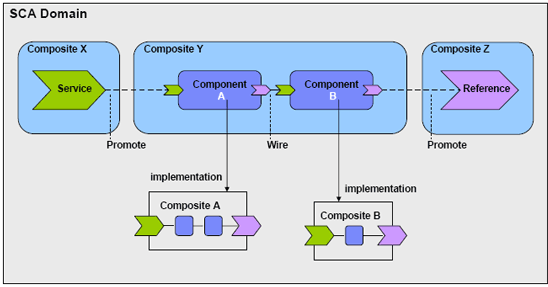
\includegraphics[width=0.8\linewidth]{Images/sca}
			\caption{SCA model example\cite{theenterprisearchitect}.}
			\label{fig:sca}
		\end{figure}
		
		\paragraph{Elaboration Language Context} The Elaboration Language is based on the SCA. Next it is presented every element that can be used and a brief description.
		\begin{itemize}
			\item \textbf{Composite} -- A composite is a set of components. These can be used to represent another components or a reference architecture.
			\item \textbf{Component} -- An entity that provides or references services. 
			\item \textbf{Property} -- Variables that can be defined inside the component and that store its characteristics.
			\item \textbf{Interface} -- A list of functions that describe a service or reference.
			\item \textbf{Service} -- Set of operations associated to a component are characterized by an interface. 
			\item \textbf{Reference} -- A service that is consumed by a component. Also characterized by an interface.
			\item \textbf{Wire} -- A bound created between a reference and a service defined by the same interface.
			\item \textbf{Implementation} -- Code block implemented in a programming language.
		\end{itemize}

	\section{Elaboration Language}
	
	\par Elaboration Language (EL) was the DSL developed by a group of students to create models, and was written using the Eclipse frameworks Xtext and Xtend. Xtext is necessary for specifying the grammar and all the other features were written using Xtend. 
	\par EL follows the Service Component Architecture specification in which everything is composed by components. The components are related through services and references to that services. 

		\subsection{Keywords}
		
		
		\begin{table}[H]
			\centering
			\caption{EL languages keywords.}
			\label{tab:keywords}
			\begin{tabular}{l|l}
				\hline 
				\textbf{Keyword} & \textbf{Description} \\
				\hline
				annotation & Defines the character that limits the annotations in the source code \\
				
				as & Rename a promoted reference or service (promote ... as ...)\\
				
				bind & Binds a reference to a service (bind ... to ...)\\
				
				compile & Indicates the top level component to compiler\\
				
				component & Defines a component \\
				
				final & Indicates that a component has a concrete elaboration \\
				
				import & Imports the content of a file \\
				
				interface & Defines a set of functions used by a service \\
				
				is & Inherits from the specified component \\
				
				language & Definition of a language \\
				
				promote & Promotes a reference or service from a subcomponent to a component \\
				
				properties: & Defines the properties of a component \\
				
				reference & Defines the reference used in a promote (promote reference ...)\\
				
				references: & Defines the references of a component \\
				
				restrict & Restriction of the values that a property can have \\
				
				service & Defines the service used in a promote (promote service ...)\\
				
				services: & Defines the services of a component \\
				
				subcomponents: & Defines the subcomponents of a component \\
				
				to & Connects a reference to a service in a bind operation (bind ... to ...)\\
				\hline
				bool, int, string, float & Properties' data types (C style) \\
				\hline
			\end{tabular}
		\end{table}
		
		\subsection{Syntax and Semantics}
		
		\par It is essential to any language to be easily understandable. In the EL context it is necessary to understand how is it possible to express the service-based models.
		\par To a better understanding it is exposed a simple model with two components in which one offers a service to another, represented in figure \ref{fig:example-diagram}.
		
		\begin{figure} [H]
			\centering
			\includegraphics[width=0.5\linewidth]{Images/diagram}
			\caption{Example diagram.}
			\label{fig:example-diagram}
		\end{figure}
		
		\par The example diagram shows an EL model, in which the \texttt{Composite} is the component from where the model is generated. In the code this is represented by the expression \texttt{compile Composite}. It is defined a \texttt{language} and both components should follow it. In the \texttt{language} definition it is indicated the annotation symbol to be used by the elaborations later. An \texttt{interface} is created with all the functions that component \texttt{C\_B} provides as services. The component \texttt{C\_A} has one property \texttt{P\_A} of the type \texttt{int} and one reference \texttt{R\_A} to the service of the other component, so this reference must follow the same interface as the respective service from \texttt{C\_B}. The component \texttt{C\_B} offers a service \texttt{S\_B} and has a property \texttt{P\_B} of the type \texttt{string} with the default value text. Finally it is declared the component \texttt{Composite} that contains the two components described above and the \texttt{bind} of the reference \texttt{R\_A} to the service \texttt{S\_B}.
		
		\begin{EL}
			//This is a comment
			compile Composite
			
			language C {
				annotation: "@"
			}
			
			interface Interface {
				func1 func2
			}
			
			/* 
			This is another comment 
			*/
			
			component C_A (C) {
				properties:
				int P_A
				references:
				Interface R_A
			}
			
			component C_B (C) {
				properties:
				string P_B : "text"
				services:
				Interface S_B
			}
			
			component Composite (C) {
				subcomponents:
				C_A a
				C_B b
				
				bind a.R_A to b.S_B
			}
		\end{EL} 			

		\subsection{Work Flow}
	
		\par To develop and use a reference architecture there must be followed a work flow, composed by four steps: modeling, elaboration, configuration and generation. Each step provides the artifacts necessary for the subjacent step, as it is possible to see in figure \ref{fig:workflow}.
		
		\begin{figure} [H]
			\centering
			\includegraphics[width=1\linewidth]{Images/workflow}
			\caption{EL Workflow.}
			\label{fig:workflow}
		\end{figure}
	
		\paragraph{Modeling} The first step consists in designing the reference architecture and, after that, writing the respective EL scripts. In some cases it is necessary to refactor the code to keep the code in concordance with the model. It is also necessary to annotate the source files so the elaborations can replace these same annotations for literal values or expressions.

		\paragraph{Elaboration} In this step are constructed Java classes to modify the code with annotations provided by the user. After the system modeling and writing all the elaboration, it is created a Java program called \textbf{Elaborator}. This program understands the complete model.

		\paragraph{Configuration} At compilation time there are generated XML files with the configuration of the reference architecture components. The User can alter these files and by that configure properties values, arrays sizes ou change which elaboration will modify the source code.

		\paragraph{Generation} After completing all the steps above, the User can execute the Elaborator and generate the new source code. The Elaborator uses all the elaborations necessary to create the code.
		
		\subsection{AbstractElaborator API}
		
		\par The AbstractElaborator API lets the user easily configure the final files. Inside the ELPackage exists one Elaboration directory that contains the elaborations and the final files are generated in another folder in the same package.
		\par This API is composed by an abstract class named \texttt{AbstractElaborator} that implements the interface \texttt{Elaborator} and offers the base to all the other elaborations.
		\par It allows the association of annotated files with the respective elaboration using the function \texttt{openAnnotatedSource}. This function opens the file so it is possible to replace the annotations in that file with strings. When it is desired to work in another file, it is just necessary to use the same function targeting another source file. When two elaborations need to work in the same file, the function to use is \texttt{openAnnotatedSharedSource}. Bellow it is shown the functions prototypes that can be used with this API.
		
		\begin{lstlisting}[language=Java]
			//Open file
			public void openAnnotatedSource (String sourcepath)
			//Open file and specify generated file folder
			public void openAnnotatedSource (String sourcepath, String targetPath)
			//Open file shared with various elaborations
			public void openAnnotatedSharedSource (String sourcepath)
		\end{lstlisting}
		
		\par After opening the file, the \texttt{replaceAnnotation} method can be used to associate annotations with an elaborator and the source file. It is possible to replace an annotation targeting another file and not the one opened before. There are four methods that provide annotation replacement which are presented bellow.
		
		\begin{lstlisting}[language=Java]
		//Replace "anotation" with the "config" value		
		public void replaceAnotation (String annotation, String config)
		//Replace "anotation" with the "config" value in "targetfile"
		public void replaceAnotation(String anotation, String config, String targetfile)
		\end{lstlisting}
		
		\par The API also provides one method \texttt{generateFinalFiles} that generates the final files with the replaced annotations. The generated files are stored into FinalFiles directory inside EL Package. If some annotations were not successfully replaced, the console prints an error to let the user know that the files were not generated.
		
		\begin{lstlisting}[language=Java]
		//Verifies if there are annotations to replace and generate final files
		public static void generateFinalFiles()
		\end{lstlisting}		
		
		\subsection{Configuration Files}
		
		\par At compilation time, a configuration file written in XML should be created for each component. The configuration files have two roles: provide properties' values and specify which elaborations should be used.
		\par The user can alter the properties' values and choose the elaboration in the XML code respective fields. The fields are automatically filled through the EL's code generation. Bellow it is presented one XML file example.
		
		\begin{EL}
		<?xml version="1.0" encoding="UTF-8"?>
		
		<component type="Generator">
			<elaboration default="SpecificGeneratorElaboratorTemplate">SpecificGeneratorElaborator</elaboration>
			<properties>
				<property type="bool" name="optimizations" default="false"> 
					<value>
						<element>true</element>
					</value>
				</property>
			</properties>
		</component>
		\end{EL}
		
		\subsection{Use Cases}
		
		\par Two actors, the designer and the user, can interact with the languages artifacts. The user differentiates
		from the designer to the extent that he not possess the technical skills to design a reference architecture.
		\par The \textbf{designer} is responsible for writing the elaboration files and the EL model design. The \textbf{user} is only responsible for the configuration of properties, if they exist and the Elaborator execution. Figure \ref{fig:use-cases} provides a brief view over each actor role.
		
		\begin{figure} [H]
			\centering
			\includegraphics[width=0.4\linewidth]{Images/use-cases}
			\caption{Use cases for the Elaboration Language.}
			\label{fig:use-cases}
		\end{figure}
		
			
	\section{Dynamic Binary Translation}
	\par Binary translation is the process of converting code for one ISA architecture to code for another. There are two types of binary translation: static and dynamic. The main difference between the two approaches is that the static translation translates the entire program before the execution and dynamic translation translates code on demand during run time. This allows the dynamic binary translation (DBT) to deal with challenges that static binary translation do not suffice \cite{b.hawkingsb.demskyd.brueningq.zhao2015}. 
	\par In this project was used a dynamic binary translation to create the model. The DBT engine translates one basic block at a time and then executes it. The translated code, as well as the source code, is cached so if one basic block is stored into the translation cache, the cache returns a hit and it is not necessary to translate it again. 
	\par The DBT engine had Intel MCS-51, also known as 8051, as the source architecture and the ARMv7-M as the target architecture. After the code refactoring, it is possible to change the source and target architecture. Although, the translation algorithm will need to be rewritten to adapt to the target architecture needs.
	
		\subsection{Source Architecture: Intel MCS-51}
		
		\par The Intel MCS-51, also known as 8051, is part of a family of 8-bit microcontrollers family developed by Intel in the '80s. It is known for being ease of programming so it is used in large scale for small projects and to instruct students. By being a Complex Instruction Set Computer (CISC) microcontroller, it offers a large set of instructions. These characteristics make it the most popular microcontroller.
		\par The 8051 only offers one memory, divided into two separated addressing spaces to data and programs. In the data memory, the inferior block is divided into three parts: the registers bank, the bit addressable area and the draft area.
		\par The Control Processing Unit (CPU) Special Function Registers (SFR) , with exception of the Program Counter (PC), are allocated into the superior part of the intern data memory.  They are:
		\begin{itemize}
			\item ACC - Acumulator.
			\item B - Used as source and target register to division and multiplication operations.
			\item Stack Pointer (SP) - Pointer to the CPU stack.
			\item Data Pointer (DPTR) - 16-bits register used to address the external data memory. Uses two bytes, the DPL (Data Pointer Low) and DPH (Data Pointer High).
			\item P0, P1, P2, P3 - Used to latch the I/o ports.
			\item Serial Data Buffer (SBUF) - Use to transmission and reception in the serial port.
			\item Program Status Word (PSW) - Contains the CPU flags.
			\item Timer Registers - The 8051 offers three timers and each has two 8-bit registers to configure. The Timer 0 uses TH0 and TL0, Timer 1 uses and TH1 and TL1 and Timer 2 uses TH2 and TL2.
			\item Capture Registers (RCAP2H, RCAP2L) - Used by Timer 2 for the capture mode.
			\item Control Registers - IP, IE, TMOD, RCON, SCON, PCON are control resisters used by the interruption system from serial port and timing sections. 
		\end{itemize}
		
		\par It is important to note that at the time, the translation algorithm only provides a emulation of the ACC, B, SP and DPTR registers.
		\par The 8051 offers five groups of instructions: arithmetic, branch, data transfer, logic and bit-oriented. Arithmetic instructions perform several tasks such as addition, subtraction, division and multiplication. Branch instructions can perform conditional and unconditional jumps. The main difference between them is that conditional jumps rely on the condition codes to verify if the branch is taken or not. Data transfer instructions move the content of one register to another. Logic instructions perform logic operations upon corresponding bits of two registers. Bit-oriented instructions are logic operations perform upon single bits\cite{mikroelektronika}.
		\par The instructions size and format vary from 1 to 3 bytes to achieve the desired output. Even the same operation may vary in instruction size depending on the operands. Looking at the addition operation (\texttt{ADD}) case, when it is desired to add an immediate value to the accumulator (\texttt{ADD A, \#immediate}), 2 bytes are used. When it is desired to add the content of a register to the accumulator (\texttt{ADD A, Rn}), only 1 byte is used. This also means that the PC will be computed differently in accordance with the instruction size.
		
		\subsection{Target Architecture: ARMv7-M \cite{armv7-m}}
		
		\par ARMv7 is documented as a set of architecture profiles. Three profiles have been defined as follows:
		\begin{itemize}
			\item ARMv7-A the application profile for systems supporting the ARM and Thumb instruction sets, and
			requiring virtual address support in the memory management model.
			\item ARMv7-R the realtime profile for systems supporting the ARM and Thumb instruction sets, and requiring physical address only support in the memory management model.
			\item ARMv7-M the microcontroller profile for systems supporting only the Thumb instruction set, and where overall size and deterministic operation for an implementation are more important than absolute performance.
		\end{itemize}
		\par While profiles were formally introduced with the ARMv7 development, the A-profile and R-profile have implicitly existed in earlier versions, associated with the Virtual Memory System Architecture (VMSA) and Protected Memory System Architecture (PMSA) respectively. ARMv7-M only supports execution of Thumb instructions.
		
		\par The introduction of Thumb-2 technology provided a balance to the ARM and Thumb instruction sets, and the opportunity for the ARM architecture to be extended into new markets, in particular the microcontroller marketplace. To take maximum advantage of this opportunity a Thumb-only profile with a new programmers’ model (a system level consideration) has been introduced as a unique profile, complementing ARM’s strengths in the high performance and real-time embedded markets.

		\par ARMv7-M processors support the following data types in memory:
		\begin{itemize}
			\item Byte -- 8 bits
			\item Halfword -- 16 bits
			\item Word -- 32 bits
		\end{itemize}
		
		\par Processor registers are 32 bits in size. The instruction set contains instructions supporting the following data
		types held in registers:
		\begin{itemize}
			\item 32-bit pointers
			\item unsigned or signed 32-bit integers
			\item unsigned 16-bit or 8-bit integers, held in zero-extended form
			\item signed 16-bit or 8-bit integers, held in sign-extended form
			\item unsigned or signed 64-bit integers held in two registers.
		\end{itemize}
		\par Load and store operations can transfer bytes, halfwords, or words to and from memory. Loads of bytes or halfwords zero-extend or sign-extend the data as it is loaded, as specified in the appropriate load instruction.
		\par The instruction sets include load and store operations that transfer two or more words to and from memory. You can load and store 64-bit integers using these instructions.
		\par When any of the data types is described as unsigned, the N-bit data value represents a non-negative integer in the range 0 to 2 N -1, using normal binary format.
		\par When any of these types is described as signed, the N-bit data value represents an integer in the range -2 N-1 to +2 N-1 -1, using two's complement format.
		\par Direct instruction support for 64-bit integers is limited, and most 64-bit operations require sequences of two or more instructions to synthesize them.
		
		\paragraph{Integer arithmetic} The instruction set provides a wide variety of operations on the values in registers, including bitwise logical operations, shifts, additions, subtractions, multiplications, and many others. These operations are defined using pseudocode, usually in one of three ways:
		\begin{itemize}
			\item By direct use of the pseudocode operators and built-in functions defined in Operators and built-in functions.
			\item By use of pseudocode helper functions defined in the main text.
			\item By a sequence of the form:
			\begin{itemize}
				\item Use of the SInt(), UInt(), and Int() built-in functions to convert the bitstring contents of the instruction operands to the unbounded integers that they represent as two's complement or unsigned integers.
				\item Use of mathematical operators, built-in functions and helper functions on those unbounded integers to calculate other such integers.
				\item Use of either the bitstring extraction operator or of the saturation helper functions of saturation to convert an unbounded integer result into a bitstring result that can be written to a register.
			\end{itemize}
		\end{itemize}
		
		\paragraph{Shift and rotate operations} The following types of shift and rotate operations are used in instructions:
		\begin{itemize}
			\item Logical Shift Left (LSL) moves each bit of a bitstring left by a specified number of bits. Zeros are shifted in at the right end of the bitstring. Bits that are shifted off the left end of the bitstring are discarded, except that the last such bit can be produced as a carry output.
			\item Logical Shift Right (LSR) moves each bit of a bitstring right by a specified number of bits. Zeros are shifted in at the left end of the bitstring. Bits that are shifted off the right end of the bitstring are discarded, except that the last such bit can be produced as a carry output.
			\item Arithmetic Shift Right (ASR) moves each bit of a bitstring right by a specified number of bits. Copies of the leftmost bit are shifted in at the left end of the bitstring. Bits that are shifted off the right end of the bitstring are discarded, except that the last such bit can be produced as a carry output.
			\item Rotate Right (ROR) moves each bit of a bitstring right by a specified number of bits. Each bit that is shifted off the right end of the bitstring is re-introduced at the left end. The last bit shifted off the the right end of the bitstring can be produced as a carry output.
			\item Rotate Right with Extend (RRX) moves each bit of a bitstring right by one bit. The carry input is shifted in at the left end of the bitstring. The bit shifted off the right end of the bitstring can be produced as a carry output.
		\end{itemize}
		
		\paragraph{Registers and execution state} The application level programmers’ model provides details of the general-purpose and special-purpose registers visible to the application programmer, the ARM memory model, and the instruction set used to load registers from memory, store registers to memory, or manipulate data (data operations) within the registers.
		\par Applications often interact with external events. A summary of the types of events recognized in the architecture, along with the mechanisms provided in the architecture to interact with events, is included in Exceptions, faults and interrupts. 
		
		\subparagraph{ARM core registers} There are thirteen general-purpose 32-bit registers (R0-R12), and an additional three 32-bit registers which have special names and usage models.
		\par \textbf{SP stack pointer} (R13), used as a pointer to the active stack. This is preset to the top of the Main stack on
		reset.
		\par \textbf{LR link register} (R14), used to store a value (the Return Link) relating to the return address from a subroutine which is entered using a Branch with Link instruction. This register is set to an illegal value (all 1’s) on reset. The reset value will cause a fault condition to occur if a subroutine return call is attempted from it. The LR register is also updated on exception
		entry.
		\par \textbf{Note:} R14 can be used for other purposes when the register is not required to support a return from
		a subroutine.
		\par \textbf{PC program counter} is loaded with the Reset handler start address on reset.
		
		\paragraph{Application Program Status Register (APSR)} The Application Program Status Register (APSR) Program status is reported in the 32-bit Application Program Status Register (APSR), where the defined bits break down into a set of flags.
		APSR bit fields are in the following two categories:
		\begin{itemize}
			\item Reserved bits are allocated to system features or are available for future expansion. Further information on currently allocated reserved bits is available in The special-purpose program status registers (xPSR) on page B1-8. Application level software must ignore values read from reserved bits, and preserve their value on a write. The bits are defined as UNK/SBZP.
			\item Flags that can be set by many instructions:
			\begin{itemize}
				\item N, bit [31]: Negative condition code flag. Set to bit [31] of the result of the instruction. If the result is regarded as a two's complement signed integer, then N == 1 if the result is negative and N = 0 if it is positive or zero.
				\item Z, bit [30]: Zero condition code flag. Set to 1 if the result of the instruction is zero, and to 0 otherwise.
				A result of zero often indicates an equal result from a comparison.
				\item C, bit [29]: Carry condition code flag. Set to 1 if the instruction results in a carry condition, for
				example an unsigned overflow on an addition.
				\item V, bit [28] Overflow condition code flag. Set to 1 if the instruction results in an overflow condition,		for example a signed overflow on an addition.
				\item Q, bit [27]: Set to 1 if an SSAT or USAT instruction changes (saturates) the input value for the signed or unsigned range of the result.
			\end{itemize}
		\end{itemize}
			
			\subsubsection{Thumb instruction set encoding}
			\par The Thumb instruction stream is a sequence of halfword-aligned halfwords. Each Thumb instruction is either a single 16-bit halfword in that stream, or a 32-bit instruction consisting of two consecutive halfwords	in that stream.
			If bits [15:11] of the halfword being decoded take any of the following values, the halfword is the first	halfword of a 32-bit instruction:
			\begin{itemize}
				\item 0b11101,
				\item 0b11110,
				\item 0b11111.
			\end{itemize}
			\par Otherwise, the halfword is a 16-bit instruction.
			
			
			\paragraph{16-bit Thumb instruction encoding} Table \ref{tab:thumb16} shows the allocation of 16-bit instruction encodings.
			
			\begin{figure} [H]
				\centering
				\includegraphics[width=0.5\linewidth]{Images/thumb16}
				\caption{Instruction encoding.}
				\label{fig:thumb16}
			\end{figure}
			
			\begin{table}[H]
				\centering
				\caption{16-bit Thumb instruction encoding.}
				\label{tab:thumb16}
				\begin{tabular}{l|l}
					\hline 
					\textbf{opcode} & \textbf{Instruction or instruction class} \\ \hline
					00xxxx & Shift (immediate), add, subtract, move, and compare \\
					010000 & Data processing \\
					010001 & Special data instructions and branch and exchange \\
					01001x & Load from Literal Pool \\
					0101xx & \multirow{3}{*}{Load/store single data item} \\
					011xxx &  \\
					100xxx &  \\
					10100x & Generate PC-relative address \\
					10101x & Generate SP-relative address \\
					1011xx & Miscellaneous 16-bit instructions \\
					11000x & Store multiple registers \\
					11001x & Load multiple registers \\
					1101xx & Conditional branch, and supervisor call \\
					11100x & Unconditional Branch \\
					\hline
				\end{tabular}
			\end{table}
			
		\paragraph{32-bit Thumb instruction encoding} Table \ref{tab:thumb32} shows the allocation of ARMv7-M Thumb encodings in this space. op1 != 0b00. If op1 == 0b00, a 16-bit instruction is encoded.
		
		\begin{figure} [H]
			\centering
			\includegraphics[width=0.95\linewidth]{Images/thumb32}
			\caption{Instruction encoding.}
			\label{fig:thumb32}
		\end{figure}

			\begin{table}[H]
				\centering
				\caption{32-bit Thumb instruction encoding.}
				\label{tab:thumb32}
				\begin{tabular}{l|l|l|l}
					\hline 
					\textbf{op1} & \textbf{op2} & \textbf{op} & \textbf{Instruction class} \\ \hline
					01 & 00xx 0xx & x & Load/store multiple \\
					01 & 00xx 1xx & x & Load/store dual or exclusive, table branch \\
					01 & 01xx xxx & x & Data processing (shifted register) \\
					01 & 1xxx xxx & x & Coprocessor instructions \\
					10 & x0xx xxx & 0 & Data processing (modified immediate) \\
					10 & x1xx xxx & 0 & Data processing (plain binary immediate)  \\
					10 & xxxx xxx & 1 & Branches and miscellaneous control  \\
					11 & 000x xx0 & x & Store single data item \\
					11 & 00xx 001 & x & Load byte, memory hints \\
					11 & 00xx 011 & x & Load halfword, unallocated memory hints \\
					11 & 00xx 101 & x & Load word \\
					11 & 00xx 111 & x & UNDEFINED \\
					11 & 010x xxx & x & Data processing (register) \\
					11 & 0110 xxx & x & Multiply, and multiply accumulate\\
					11 & 0111 xxx & x & Long multiply, long multiply accumulate, and divide \\
					11 & 1xxx xxx & x & Coprocessor instructions \\
					\hline
				\end{tabular}
			\end{table}
		
			
	\subsection{Architectural Model}
	\par Figure \ref{fig:block} represents the model of the DBT engine. The execution flows as followed: a source code is loaded into a source code cache. This cache exists so that only the basic block that is being worked is loaded into RAM memory for quicker access. The DBT engine accesses the source code cache and translates the basic block which is then stored into Translation Cache. The code stored into this cache is native code for the target and ready to execute\cite{f.salgadoj.mendesa.tavaresm.ekpanyapong}.
		
	\begin{figure} [H]
		\centering
		\includegraphics[width=0.65\linewidth]{Images/block}
		\caption{Dynamic Binary Translation architectural model.}
		\label{fig:block}
	\end{figure}


	\section{Resources}
	
		\par For the concretization of this project, there will be used some hardware and software. These are presented next.

		\subsection{Hardware}
		
			\par Here is described the hardware used during the project. All of it was chosen for availability reasons. 

			\paragraph{SmartFusion2 Advanced Development Kit}
			
			\par Microsemi's SmartFusion2 Advanced Development Kit offers a full featured device SmartFusion2 system-on-chip FPGA. This device inherently integrates reliable flash-based FPGA fabric, a Cortex-M3 processor, digital signal processing (DSP) blocks, static random-access memory (SRAM), embedded nonvolatile memory (eNVM), and industry-required high-performance communication interfaces—all on a single chip \cite{microsemi}. 
			\par This device is used to run the generated sources files so its veracity is verified. 
			
			\begin{figure} [H]
				\centering
				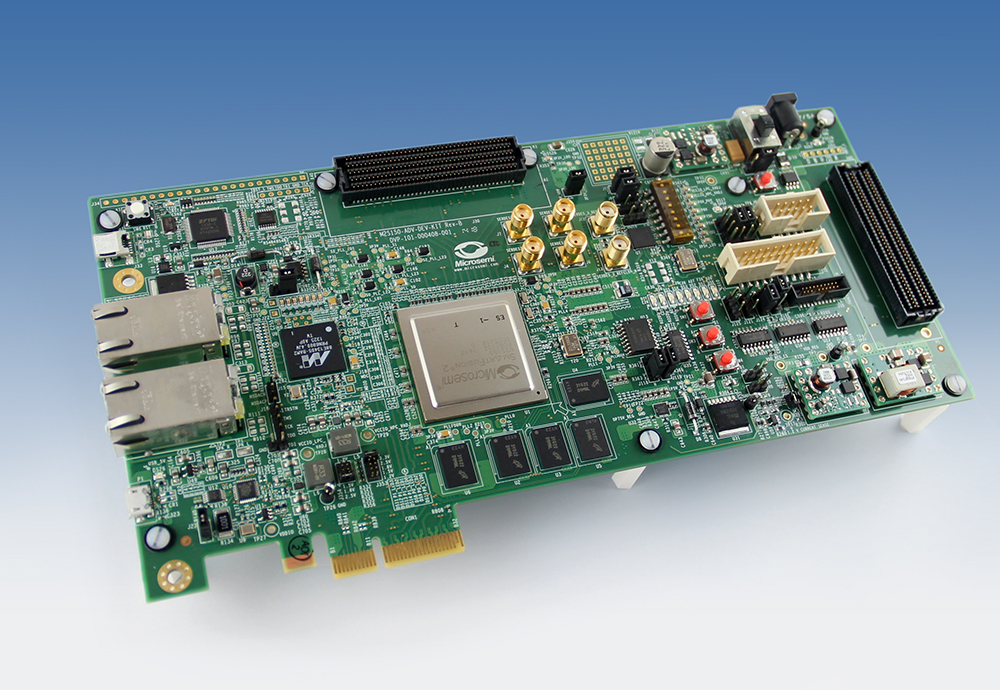
\includegraphics[width=0.5\linewidth]{Images/microsemi}
				\caption{SmartFusion2 Advanced Development Kit.}
				\label{fig:microsemi}
			\end{figure}

		\paragraph{Debugger} The debugger is used to communicate with the device and receive important information about the execution. It has a JTAG interface to interact with the processor and USB to interact with the computer, and supports all ARM 7/9/11, Cortex. In this project it is used the J-Link Segger. 
		
			\begin{figure} [H]
				\centering
				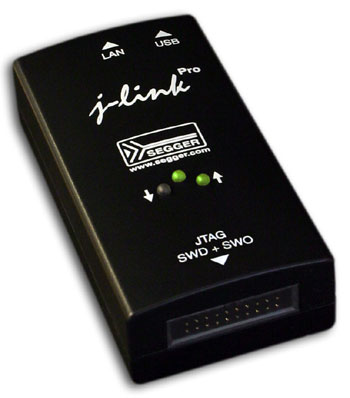
\includegraphics[width=0.3\linewidth]{Images/jlink}
				\caption{Segger J-Link.}
				\label{fig:jlink}
			\end{figure}

		\subsection{Software}
		
		\par The software used in this project was available to download by the developers in internet. 
		
			\paragraph{Eclipse}
			
			\par Eclipse Integrated Developing Environment (IDE) has first developed to program JAVA applications, but its plugins system provides the programming in various languages. This will be used to write the EL script, the elaborations and to generate code.

			\begin{figure} [H]
				\centering
				
\includegraphics[width=0.3\linewidth]{Images/eclipse}
				\caption{Eclipse logo.}
				\label{fig:eclipse}
			\end{figure}

			\paragraph{Understand} This software is used to perform the code analysis. The source files are used to create dependences graphs between modules. Is used to validate the code refactoring. 
			
			\begin{figure} [H]
				\centering
				
\includegraphics[width=0.3\linewidth]{Images/understand}
				\caption{Understand logo.}
				\label{fig:understand}
			\end{figure}
			
			\paragraph{IAR Workbench} IAR Worksbench is an IDE used to program many platforms. This chosen platform is the ARM based. This software was used to compile the source code and validate the code generation.
			
			\begin{figure} [H]
				\centering
				
\includegraphics[width=0.2\linewidth]{Images/iar.jpg}
				\caption{IAR logo.}
				\label{fig:iar}
			\end{figure}

	\section{Implementation Plan}
	
	\par The first task was the study of the dynamic binary translator to get more familiar with the algorithm and completely understand it and its characteristics. The group's objective is to model the code generation, so this part will be studied more deeply.
	\par The second task was the study of the EL framework, where the reference architecture will be implemented following the SCA method.
	\par The third task was the implementation of the reference architecture in the framework and the code refactoring so it will fit the model. 
	\par The fourth task was writing the correspondent EL scripts, annotate the source code and write the elaborations. This will make the code configurable.
	\par It will also be necessary to prepare all the presentations, reports and poster in the project domain.
	
	\begin{figure} [H]
		\centering
		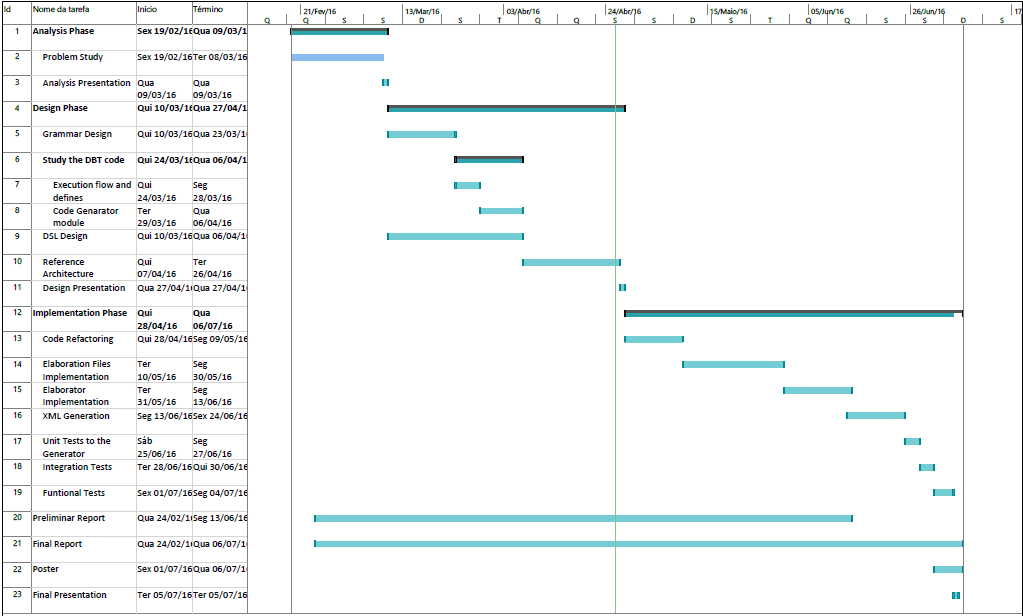
\includegraphics[width=1\linewidth]{Images/gantv2}
		\caption{Gantt's Diagram.}
		\label{fig:gantt}
	\end{figure}
	


%END ANALYSIS CHAPTER
%-------------------------------------------
%START DESIGN CHAPTER

\chapter{Design}

	\par In this section the dynamic binary translator program is analyzed at detail. Then, the reference architecture is constructed in order to allow the systems configuration. 
	\par The dependencies graph will be generated using the Understand software. After this analysis will be decided if the code needs to be refactored in order to be in accordance with the model. 
	
	\section{Code Analysis}
	
	\par The primary source files assigned to the group were not written following a reference architecture. So, the first task is to understand how to code should be organized to be modular. This means that is necessary to identify components, services and references and how do they connect to each other.
	\par The first step is to analyze the \texttt{main} file. It is created an object of the \texttt{DBTEngine} type and the code size is passed as argument to the initialization method. Hereupon is only necessary to run the translator.
	\par To start the translation, there must be code into translation cache. If the source PC does not have a Translation Cache entry, a new entry in Translation Cache is added. Then, the entry location is saved as "next to execute" and a prolog is generated. The prolog pushes all the necessary registers and the Link Register (LR) to stack. After the prolog generation, the code cache is accessed and the next instruction is fetched. 
	\par Then the decoding stage starts and the raw code is treated in order to get the opcode and operands of the fetched instruction. In the end of decode, it is pointed to the next instruction and the target code is generated. It is important to note that one decoded instruction may result in many more target instructions due to ISA incompatibility. 
	\par At this point, if the instruction is a control flow instruction, the algorithm fetches another instruction, decodes it and generates the raw binary for the target again. If not, the epilog is generated and the used registers as well as the PC are poped from stack. After epilog the code is executed and goes to the begin of the algorithm.
	\par This situation happens when the source PC does not have a Translation Cache entry. When this entry exists, the code address is accessed and set as "next to execute", then executed. The flowchart for this algorithm is presented on figure \ref{fig:flowchart-codeanalysis}.
	
	\begin{figure} [H]
		\centering
		\includegraphics[width=0.5\linewidth]{Images/flow-codeanalysis}
		\caption{Translation algorithm.}
		\label{fig:flowchart-codeanalysis}
	\end{figure}	
	
	\par With this analysis it was possible to identify all the necessary components and its interfaces that will be later exposed in the reference architecture and to verify that the primary code needed to be refactored.

	\par The code was also analyzed using the Understand software to prove that the refactor is needed so the code is in accordance with the reference architecture. The resulting graph is presented in figure \ref{fig:understand1}.
	
	\begin{figure} [H]
		\centering
		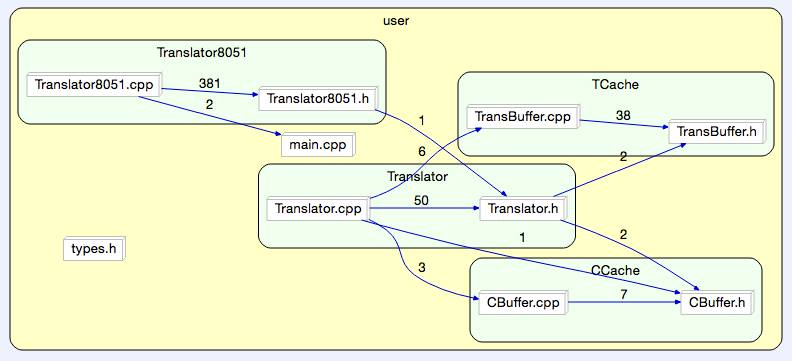
\includegraphics[width=0.6\linewidth]{Images/refactor1.jpg}
		\caption{First analysis done using the Understand software.}
		\label{fig:understand1}
	\end{figure}

	\section{Code Refactoring}
	Code refactoring is the process of reorganizing and restructuring of existing code in source files without changing its external behavior. To keep the behavior there are some decisions that need to be made that may introduce overhead in the computation time, which is unwanted in an embedded system. That is why the overhead introduced by refactoring should be as minimal as possible.
	
	Code Refactoring can make improvements in code or simply make the code easier to read and understand.
	In this case, the objective of code refactoring is to make it easier to model. This objective can improve also the maintainability because the code will be more readable. The objectives are conceived by dividing the code in different sources and classes, with which one representing a key part of the DBT.
	
	The original code does not have many divisions. The part of code responsible for decoding the operands is done in the same file that the part that is responsible of generating the code. 
	This is shown in the next diagram (Figure \ref{fig:uml1}).
	
	\begin{figure} [H]
		\centering
		\includegraphics[width=0.8\linewidth]{Images/UMLDBT}
		\caption{Class Diagram of DBT}
		\label{fig:uml1}
	\end{figure}
	
	The code's division will create new classes, to make a separation from the code that is related to the source architecture and the decoding of instructions from the source architecture, to the code that is related to the target architecture and the generating of code to that architecture.
	This refactoring and separation will improve the process of switching from architecture to another. This is accomplished because the designer doesn't need to alter complex file with all the functions of target and source architecture, but only the file with the specific functions. 
	
	The changes in code are described in next paragraphs:
	
	\paragraph{main.cpp}
	In the file \texttt{main.cpp}, it's only needed to rearrange the calls to the methods from the main class because in the initial code, the classes had the same names as after refactoring.
	
	\paragraph{DBTEngine}
	The translator class was renamed \texttt{CDBTEngine} because is the core class of the DBT that initializes and starts the translation. 
	
	\paragraph{CBuffer}
	The only change in this file was to add the macro \texttt{fetch} to it. The macro \texttt{fetch} was previously in the class translator that was the class that had methods to start and initialize the translation. The macro gives access to the content of the Code Buffer so it makes more sense to be defined in \texttt{CBuffer}, that is were the Code Bufeer is initialized and loaded with code.
	
	\paragraph{TransBuffer}
	Some minor change was done in the TransBuffer Class to be in accordance with the other classes.
	
	\paragraph{SourceArchitecture}
	The Class Source Architecture was introduced to separate the decoder from the generator. It includes all the methods that the decode should implement.
	
	\paragraph{SourceArch\_8051}
	SourceArch\_8051 Class is the specific class that decodes instructions from the 8051 architecture. The designer needs to change this class if we wants to switch architecture.  
	
	\paragraph{TargetArchitecture}
	The Class Target Architecture is a abstract class with the methods responsible for code generation. It has all the methods as virtual to be implemented in the derivate class that is specific to an Architecture.
	
	\paragraph{TargetArch\_CortexM3}
	TargetArch\_CortexM3 Class is where the Generator methods are implemented and this file should be altered if it is wanted switch to another target architecture.  
	
	\paragraph{Defines}
	The defines were separated in different files. The defines concerning the Source Architecture were put in the file \texttt{SourceDefines.h} and those defines that were related to the Target Architecture in the file \texttt{TargetDefines.h}. The file \texttt{types.h} continues to exist with only the global defines.
	
	The figure \ref{fig:refactoring} shows the relations and division of the classes.
	
	\begin{figure} [H]
		\centering
		\includegraphics[width=0.75\linewidth]{Images/newclasses}
		\caption{Code Refactoring Class Diagram.}
		\label{fig:refactoring}
	\end{figure}	
	
	
	\section{Code Generation}
	The Code Generation is the last stage of code's translation in DBT. After decoding the source instruction, code generation is called to generate code that follows Target Instruction Set Architecture. The behavior of instructions is reproduced through an Intermediate Representation. The use of an Intermediate Representation provides advantages like increased abstraction and add the possibility of retargeting.
	
	In this project the Intermediate Representation is defined as set of functions that should be redefined for each target Instruction Set Architecture. This method is based on QEMU Tiny Code Generator \cite{fabricebellard}. Each of this functions generate the corresponding code to the translation cache. 
	
	The figure \ref{fig:generation} represents a example of the translation stages in DBT (instruction decoding and code generation) for the source architecture 8051 and to target architecture Cortex M3.
	
	\begin{figure} [H]
		\centering
		\includegraphics[width=0.7\linewidth]{Images/codegeneration}
		\caption{Code Generation}
		\label{fig:generation}
	\end{figure}	
	
	The 8051 code has a \texttt{INC A} instruction. The decoder has, for each instruction, a template of intermediate representation that is a conjunct of functions that should be call in order to generate the corresponding code for that instruction from source architecture. In this case, the intermediate representation for  the \texttt{INC A} instruction is load of a byte from the Accumulator of the source architecture to the temporary register, then add one to that temporary and finally store that temporary register in the accumulator. The code generation process is done inside of each of these functions that generate the corresponding instructions for each intermediate representation.
	
	Inside of each function there is temporary variables. And each function applies a series of masks with the opcode and put the registers that function receives in the right place in the instruction. After this process are concluded the temporary variables have the corresponding instruction for the target architecture. The next step, inside the function, is to put that temporary variables in the translation cache for later execution. As observed, the functions are specific for an architecture, because they generate the specific instruction for an architecture defined by the designer. 

	As can be observed in the following schematic, these type of intermediate representation has two types of functions:
	
	\begin{figure} [H]
		\centering
		\includegraphics[width=0.8\linewidth]{Images/functions}
		\caption{Intermediate Representation Function types}
		\label{fig:genfunctions}
	\end{figure}
	
	The table \ref{IRTable} represents the functions that are used to generate code. The main objective is  to clarify and show the series of functions that are involved in this part of the DBT. 
	
	With the observation of the table, it is possible to verify that the intermediate representation has a vast number of functions. These functions represent basic instructions or operations, for example, addition, logic or, load, store and so on.
	
	The two functions that are most used are load and store because to make some alteration in a variable located in memory, it is need to load that variable before it's used. After the operation complete it is necessary to store again in the same memory position the result.
	
	The first two gen functions in table are relevant functions because they are needed to save and restore the context before and after a basic block.
	
	\begin{table}[H]
		\caption{Code Generation Functions}
		\label{IRTable}
		\centering
		\begin{tabular}{|l|p{10cm}|}
			\hline
			\rowcolor[HTML]{C0B0C1} 
			\textbf{Functions}	    		  &	\textbf{Description}\\ \hline
			gen\_prolog			    		  &	Saving the value and state of the registers \\ \hline 
			gen\_epilog			    		  &	Restoring the value and state of the registers \\ \hline 
			gen\_blx		    	          &	Branch with link \\ \hline 
			gen\_PUSH, gen\_POP               &	Push or pop multiple registers \\ \hline 
			gen\_cmp, gen\_cmpi 	          &	Compares two values\\ \hline 
			gen\_it					          & If then	\\ \hline 
			gen\_cje, gen\_cjei 	          & Compare two values and jump if they are equal	\\ \hline 
			gen\_cjne, gen\_cjnei		      & Compare two values and jump if they are not equal	\\ \hline 
			gen\_writePC, gen\_writePCreg     & Alter the Value of Program Counter\\ \hline 
			gen\_mov 					      & Moves a value from a register to another\\ \hline 
			gen\_movi 						  & Moves a immediate value to a register \\ \hline
			gen\_ld8, gen\_ld16, gen\_ldi8	  & Loads a value from memory to a register\\ \hline 
			gen\_st8, gen\_st16, gen\_sti8    &	Stores a value from registers into the memory\\ \hline 
			gen\_ld\_bit                      &	Loads a bit from memory\\ \hline 
			gen\_st\_bit                      &	Stores a bit in the memory\\ \hline 
			gen\_add gen\_addi				  &	Addition \\ \hline 
			gen\_sub, gen\_subi				  &	Subtract \\ \hline 
			gen\_div						  &	Division \\ \hline 
			gen\_mul					      &	Multiplication \\ \hline 
			gen\_not						  &	Negate a register\\ \hline 
			gen\_or, gen\_ori				  &	Or logic \\ \hline 
			gen\_and, gen\_andi				  &	And logic \\ \hline 
			gen\_xor						  &	Xor logic \\ \hline 
			gen\_shri, gen\_shli			  &	Logic Shift right and logic shift left \\ \hline 
			gen\_orShl 						  &	Logic or add shift left\\ \hline 
			helper\_ret 					  & Reproduces the steps that source architecture has when returning from a subroutine	\\ \hline 
			helper\_call 					  & Reproduces the steps that source architecture has when calling a subroutine	\\ \hline 
			helper\_DA						  &	Adjust accumulator after a addition \\ \hline 
		\end{tabular}
	\end{table} 
	
	As mentioned before, the decoding and code generation are parts of the translation that are tightly correlated. That connection between the two parts is made through the "gen" functions, in other words the functions of the intermediate representation are called in the decode in order to generate code.
	
	Another thing that can be concluded is that the generator part of the translation is related to the target architecture. This happens, because to generate code it is need to know the registers and opcodes of the target architecture.
	
	At the same time, the code generator also needs some informations from the source architecture, like for example, the Program Counter.  On the other hand, the code generation needs to have access to the memory of the source architecture to get and set the registers that are mapped in memory and also the memory contents of other positions. The memory of the source architecture is simulated inside of the target memory.  Thus, the code generation only needs to know where that memory is located.
	
	Other aspect to highlight is that the code generation writes the result of generation in the translation cache.
	
	These relationships above cited will be explained during this report, since to model the code we first need to understand the relationships that code generation has with the other parts of the code.


	\section{Reference Architecture}
	
	\par This section explains each of the reference architecture's component and its properties and interfaces. The name notation used indicates that all the references are started with \texttt{r\_} and all the services start with \texttt{s\_}.
	\par The symbols notation is show in figure \ref{fig:caption}.
	
	\begin{figure} [H]
		\centering
		\includegraphics[width=0.1\linewidth]{Images/arch-ref/caption}
		\caption{Symbols used in the reference architecture model.}
		\label{fig:caption}
	\end{figure}

	
		\subsection{DBT}
		
		\par The composite \texttt{DBT} includes all the other components and composites of the dynamic binary translator reference architecture. It references one service of \texttt{DBTEngine} -- \texttt{r\_Engine} -- and two references \texttt{r\_MemSizes} of the service \texttt{s\_MemSizes} of the architecture components. This top level also has one property called \texttt{measure} which is a boolean and activates/deactivates functions to measure the number of cycles that the program executes.
		
		\begin{figure} [H]
			\centering
			\includegraphics[width=1\linewidth]{Images/arch-ref/ref-arch}
			\caption{Reference Architecture of a dynamic binary translator.}
			\label{fig:ref-arch}
		\end{figure}	
	
		\subsection{SourceCluster}
		
		\par The composite \texttt{SourceCluster} includes two components for source architecture and decoder -- \texttt{SourceArch} and \texttt{Decoder} -- and one composite for the source environment -- \texttt{SourceEnv}. It has no services, references or properties.
		
		\begin{figure} [H]
			\centering
			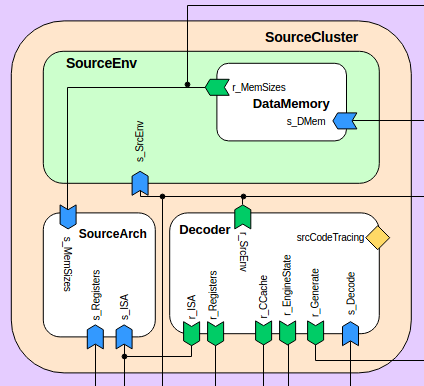
\includegraphics[width=0.6\linewidth]{Images/arch-ref/SourceCluster}
			\caption{SourceCluster composite.}
			\label{fig:SourceCluster}
		\end{figure}
		
			\subsubsection{SourceArch}
			
			The component \texttt{SourceArch} contains the necessary information about the source architecture. It only offers services -- \texttt{s\_MemSizes} that include the external, internal and data memory sizes as well the heap and stack sizes, \texttt{s\_Registers} that informs about the architecture registers and \texttt{r\_ISA} that includes the functions to get the word size, get the PC size and get the number of bits of the opcode. It does not contains properties.
			
			\begin{figure} [H]
				\centering
				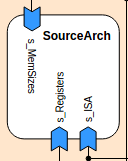
\includegraphics[width=0.25\linewidth]{Images/arch-ref/SourceArch}
				\caption{SourceArch component.}
				\label{fig:SourceArch}
			\end{figure}
		
			\subsubsection{SourceEnv}
			
			\par The composite \texttt{SourceEnv} has one service -- \texttt{s\_SrcEnv} that is used to get and set the PC and reset the environment. It does not has references or properties.
			
			\begin{figure} [H]
				\centering
				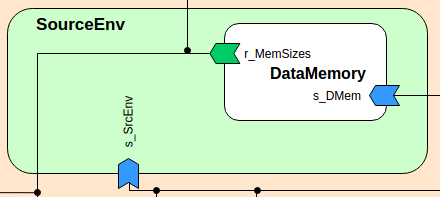
\includegraphics[width=0.5\linewidth]{Images/arch-ref/SourceEnv}
				\caption{SourceEnv composite.}
				\label{fig:SourceEnv}
			\end{figure}
		
				\subsubsubsection{DataMemory}
				
				\par \texttt{DataMemory} offers one service -- \texttt{r\_DMem} that allows the other components to read and write into data memory -- and one reference to the \texttt{s\_MemSizes} service from \texttt{SourceArch}. It has no properties.
		
				\begin{figure} [H]
					\centering
					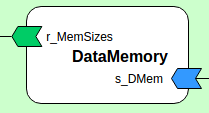
\includegraphics[width=0.3\linewidth]{Images/arch-ref/DataMemory}
					\caption{DataMemory component.}
					\label{fig:DataMemory}
				\end{figure}
		
			\subsubsection{Decoder}
			
			\par The component \texttt{Decoder} has six references -- \texttt{r\_ISA} to get the word and PC size and the number of bits of the opcode of the \texttt{SourceArch}, \texttt{r\_Registers} to get the register from \texttt{SourceArch}, \texttt{r\_SrcEnv} to get and set PC, \texttt{r\_CCache} to access the code stored into \texttt{CodeCache}, \texttt{r\_EngineState} from \texttt{DBTEngine} to access the pointers \texttt{eoBB} (end of Basic Block) and \texttt{EoExec} (end of Execution) and \texttt{r\_Generate} to call the functions provided by the \texttt{Generator} -- and one service -- \texttt{s\_Decode} that offers the decoding functions. It has one property \texttt{srcCodeTracing} to let the user decide if he wants to print the decoded instruction in serial port. This can be used as debug. 
			
			\begin{figure} [H]
				\centering
				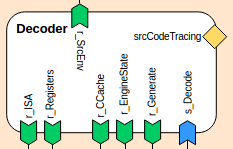
\includegraphics[width=0.45\linewidth]{Images/arch-ref/Decoder}
				\caption{Decoder component.}
				\label{fig:Decoder}
			\end{figure}			
		
		
		\subsection{TargetCluster}
		
		\par The composite \texttt{TargetCluster} has two components -- \texttt{Generator} and \texttt{TragetArch}. It does not contains services, references or properties.
		
		\begin{figure} [H]
			\centering
			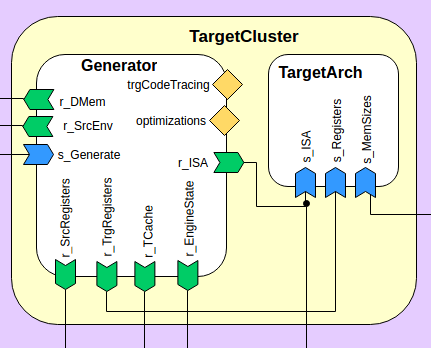
\includegraphics[width=0.6\linewidth]{Images/arch-ref/TargetCluster}
			\caption{TargetCluster composite.}
			\label{fig:TargetCluster}
		\end{figure}
		
			\subsubsection{TargetArch}
			
			\par The \texttt{TargetArch} component includes the three services from target architecture -- \texttt{s\_ISA} to get word and PC size and to get number of bits from opcode, \texttt{s\_Registers} and \texttt{s\_MemSizes} the size of the memories, heap and stack. No properties and references exist in this component.
			
			\begin{figure} [H]
				\centering
				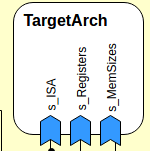
\includegraphics[width=0.25\linewidth]{Images/arch-ref/TargetArch}
				\caption{TargetArch component.}
				\label{fig:TargetArch}
			\end{figure}
		
			\subsubsection{Generator}
			
			\par The \texttt{Generator} component is responsible for the code generation for target architecture. It has seven references -- \texttt{r\_DMem} to read from data memory, \texttt{r\_SrcEnv} to access PC, \texttt{r\_SrcRegisters} to get the registers from source architecture, \texttt{r\_TrgRegisters} to get the registers from target architecture, \texttt{r\_TCache} to store the generated instructions in Translation Cache, \texttt{r\_EngineState} to access the \texttt{eoBB} (end of Basic Block) and \texttt{eoExec} (end of execution) pointers and \texttt{r\_ISA} to get word and PC size as well as the number of bits from the opcode -- and one service -- \texttt{s\_Generate} is responsible for code generation. It also contains two properties -- \texttt{trgCodeTracing} to let the user decide if he wants to print the generated instructions in serial port and \texttt{optimizations} to activate the code generation optimizations.  
			
			\begin{figure} [H]
				\centering
				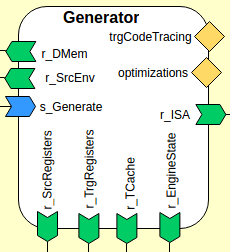
\includegraphics[width=0.35\linewidth]{Images/arch-ref/Generator}
				\caption{Generator component.}
				\label{fig:Generator}
			\end{figure}
			
		\subsection{CodeCache}
		
		\par The \texttt{CodeCache} stores the code to be translated. It has one reference -- \texttt{r\_ISA} to get word and PC size as well as the number of bits from the opcode -- and one service -- \texttt{s\_CCache} to provide the fetch and the load of instructions, add tags and get last and current translation address. The property \texttt{CCache\_Size} lets the user configure the cache size. 
		
		\begin{figure} [H]
			\centering
			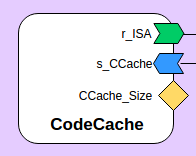
\includegraphics[width=0.3\linewidth]{Images/arch-ref/CodeCache}
			\caption{CodeCache component.}
			\label{fig:CodeCache}
		\end{figure}
		
		\subsection{TranslationCache}
		
		\par The \texttt{TranslationCache} stores the translated code to be executed. It has one reference -- \texttt{r\_ISA} to get word and PC size as well as the number of bits from the opcode -- and one service -- \texttt{s\_TCache} to store the translated code, add tags and get last and current translation address. The property \texttt{CCache\_Size} lets the user configure the cache size. 
		
		\begin{figure} [H]
			\centering
			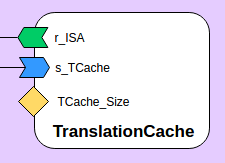
\includegraphics[width=0.3\linewidth]{Images/arch-ref/TranslationCache}
			\caption{TranslationCache component.}
			\label{fig:TranslationCache}
		\end{figure}
		
		\subsection{DBTEngine}
		
		\par The composite \texttt{DBTEngine} contains the \texttt{Translator} and the \texttt{Executor} components. It references four services -- \texttt{r\_Translate} connected to a service from \texttt{Translator}, \texttt{s\_SrcEnv} that is used to get and set the PC and reset the environment, \texttt{s\_CCache} to fetch instructions, \texttt{r\_Execute} to bind to service from \texttt{Executor} and \texttt{r\_TCache} to access the translated code -- and three services -- \texttt{s\_Engine} to initialize and start the program, \texttt{s\_CurrBBExec} that points to the basic block being executed and \texttt{s\_EngineState} to access the pointers \texttt{eoBB} (end of Basic Block) and \texttt{EoExec} (end of Execution). It does not contains properties.
		
		\begin{figure} [H]
			\centering
			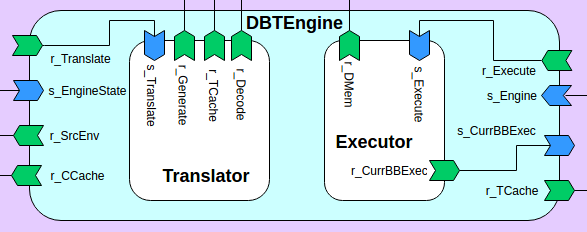
\includegraphics[width=0.7\linewidth]{Images/arch-ref/DBTEngine}
			\caption{DBTEngine composite.}
			\label{fig:DBTEngine}
		\end{figure}
		
			\subsubsection{Translator}
			
			\par The \texttt{Translator} component offers one service -- \texttt{s\_Translate} -- and three references -- \texttt{r\_Generate}, \texttt{r\_TCache} to access code in \texttt{TranslationCache} and \texttt{r\_Decode} -- and one service -- \texttt{s\_Translate}. It does not contains properties. 
				
			\begin{figure} [H]
				\centering
				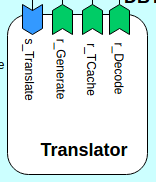
\includegraphics[width=0.3\linewidth]{Images/arch-ref/Translator}
				\caption{Translator component.}
				\label{fig:Translator}
			\end{figure}
			
			\subsubsection{Executor}
			
			\par The \texttt{Executor} component has two references -- \texttt{r\_DMem} to read and write into data memory and \texttt{r\_currBBExec} to access the basic block being executed -- and one service -- \texttt{s\_Execute}. It offers no properties.

			\begin{figure} [H]
				\centering
				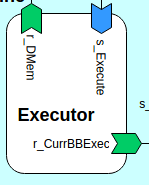
\includegraphics[width=0.3\linewidth]{Images/arch-ref/Executor}
				\caption{Executor component.}
				\label{fig:Executor}
			\end{figure}
			
		\subsection{Interfaces}\label{sec:interfaces}
		
		\par The interfaces make possible for components to connect between each other. To connect two components, one most have one reference of a given interface and the other must have a service of the same interface.

			\subsubsection*{i\_ISA}
			
			\par The \texttt{i\_ISA} interface has three functions:
			\begin{itemize}
				\item getWordSize -- the word size is a characteristic of the architecture and it's necessary to encode the instructions correctly,
				\item PCSize -- the Program Counter size may be different of the word size, so this function is also necessary for the correct encoding,
				\item nBitsOpcode -- the number of bit of the opcode may vary. Looking at the Thumb specification, the opcode size is different when using the 16-bit and 32-bit encoding. 
			\end{itemize}
			
			\begin{EL}
			interface i_ISA {
				getWordSize	
				PCSize
				nBitsOpcode
			}
			\end{EL} 
			
			\subsubsection*{i\_MemSizes}	
			
			\par The \texttt{i\_MEMSizes} interface has five functions:
			\begin{itemize}
				\item xDataMemSize -- indicates the size of the external data memory,
				\item DataMemSize -- indicates the size of the internal data memory,
				\item MemSize -- indicates the size of the code memory,
				\item HeapSize -- indicates the size of the heap,
				\item StackSize -- indicates teh size of the stack.
			\end{itemize}
			
			\begin{EL}
			interface i_MemSizes{
				xDataMemSize 	
				DataMemSize 	
				MemSize			
				HeapSize			
				StackSize		
			}
			\end{EL} 	

			\subsubsection*{i\_Registers}
			
			\par The \texttt{i\_Registers} interface does not have functions associated, but it should return the available registers for a given architecture.
			
			\begin{EL}
			interface i_Registers {
			}
			\end{EL}
			
			\subsubsection*{i\_SrcEnv}	
			
			\par The \texttt{i\_SrcEnv} interface has three functions:
			\begin{itemize}
				\item getPC -- to get the value stored in the Program Counter,
				\item setPC -- to set the value of the Program Counter,
				\item envReset -- to reset the environment.
			\end{itemize}
			
			\begin{EL}
			interface i_SrcEnv {
				getPC
				setPC
				envReset
			}
			\end{EL}
			
			\subsubsection*{i\_TCache}
			
			\par The \texttt{i\_TCache} interface has five functions:
			\begin{itemize}
				\item addTag -- add a tag to a given instruction,
				\item getTransAddr -- get the translated instruction address,
				\item getLastTransAddr -- get the last translated instruction address, 
				\item getCurrInsAddr -- get the current instruction address,
				\item cacheCode -- stores the code into cache.
			\end{itemize}
		
			\begin{EL}
			interface i_TCache {
				addTag 			
				getTransAddr		
				getLastTransAddr 	
				getCurrInsAddr	
				cacheCode		
			}
			\end{EL}
			
			\subsubsection*{i\_CCache}
			
			\par The \texttt{i\_CCache} interface has two functions:
			\begin{itemize}
				\item fetch -- to retrieve the instruction address from code cache,
				\item load -- to load code to translate from code cache.
			\end{itemize}
			
			\begin{EL}
			interface i_CCache {
				fetch	
				load
			}
			\end{EL}
			
			\subsubsection*{i\_DMem}
			
			\par The \texttt{i\_DMem} interface has two functions:
			\begin{itemize}
				\item readDataMemory -- to read data from data memory,
				\item writeDataMemory -- to write data into data memory.
			\end{itemize}
			
			\begin{EL}
			interface i_DMem {
				readDataMem	 	
				writeDataMem
			}
			\end{EL}			
			
			\subsubsection*{i\_Decode}
			
			\par The \texttt{i\_Decode} interface has one function:
			\begin{itemize}
				\item decode -- to use the instruction decoding functions.
			\end{itemize}
			
			\begin{EL}
			interface i_Decode {
				decode 
			}
			\end{EL}	
					
			\subsubsection*{i\_Generate}
			
			\par The \texttt{i\_Generate} interface has fourty eight functions. All of its purposes is to generate binary code for the target architecture.
			
			\begin{EL}
			interface i_Generate {
				helper_ret	helper_call	helper_xmem_range	
				helper_CC_lazyEv_SNIFFER_BACKDOOR	helper_DA	
				helper_debug
				gen_assemble_lazyEv_param
				gen_helper	
				gen_brkp  	gen_blx
				gen_PUSH  	gen_POP
				gen_cmp 	gen_cmpi
				gen_it  
				gen_cje  	gen_cjne	gen_cjei  	gen_cjnei
				gen_writePC gen_writePCreg
				gen_mov  	gen_movi
				gen_ld8  	gen_ld16  gen_ldi8
				gen_st8	 	gen_st16  gen_sti8
				gen_ld_bit  gen_st_bit
				gen_add  	gen_addi
				gen_sub  	gen_subi
				gen_div  	gen_mul
				gen_not
				gen_or  	gen_ori
				gen_and  	gen_andi
				gen_xor
				gen_shri 	gen_shli
				gen_orShl
				gen_prolog  gen_epilog
			}
			\end{EL}
			
			\subsubsection*{i\_Translate}
			
			\par The interface \texttt{i\_Translate} has one function:
			\begin{itemize}
				\item translate -- to translate the source code. It is not the same as decode or generate code.
			\end{itemize}
			
			\begin{EL}
			interface i_Translate{
				translate 
			}
			\end{EL}

			\subsubsection*{i\_CurrBBExec}
			
			\par The interface \texttt{i\_CurrBBExec} has one function:
			\begin{itemize}
				\item currBBExecPtr -- to access the pointer to the current basic block being executed.
			\end{itemize}
			
			\begin{EL}
			interface i_CurrBBExec{
				currBBExecPtr
			}
			\end{EL}
			
			\subsubsection*{i\_Execute}
			
			\par The interface \texttt{i\_Execute} has one function:
			\begin{itemize}
				\item execute -- to execute the translate code into the target machine.
			\end{itemize}
			
			\begin{EL}
			interface i_Execute{
				execute
			}
			\end{EL}
			
			\subsubsection*{i\_Engine}
			
			\par The interface \texttt{i\_Engine} has two functions:
			\begin{itemize}
				\item initTranslator -- to initialize the translator with code size and code location,
				\item runDBT -- to initialize the translation and posterior execution.
			\end{itemize}
			
			\begin{EL}
			interface i_Engine{
				initTranslator
				runDBT
			}
			\end{EL}
			
			\subsubsection*{i\_EngineState}		
			
			\par The interface \texttt{i\_EngineState} has three functions:
			\begin{itemize}
				\item eoBB -- access the pointer to the end of basic block,
				\item eoExec -- access the pointer to the end of execution,
				\item pSourceProgMem -- to access the source program memory.
			\end{itemize}	
			
			\begin{EL}
			interface i_EngineState{
				eoBB
				eoExec
				pSourceProgMem
			}
			\end{EL}	

	\section{Test Plans}
	
	\par Tests are used to validate all the work. The needed tests are presented bellow.
	
	\paragraph{Single elaboration test} This test verifies the modeling tool and consists in creating a dummy component or composite, its reference architecture and elaboration. The expected result is the annotations' replacement associated with the source files.  
	
	\paragraph{Integration test} This test consists in reunite all the elaborations and generate the full program. It is used the complete reference architecture of the DBT, written in Elaboration Language, and execute the elaborator to generate the source files of the BDT. All the properties are used with default values.
		
	\paragraph{Properties test} This test is performed after the other two. Its purpose is to verify if the configuration is doing the proper alteration of the properties' values.
	
	\paragraph{Execution test} The last test purpose is to test the generated source files. Then, this files are use to create a project in IAR Workbench and compiled. The binary code is flashed into the SmartFusion2 Advanced Development Kit and executed. If this test succeeds, the project is also successful. 
%END DESIGN CHAPTER
%-------------------------------------------
%START IMPLEMENTATION CHAPTER

\chapter{Implementation Phase}

	\section{Elaboration Language Scripts}
	
	\par This section shows the concretization of the previously presented reference architecture into EL scripts. Not all scripts will be shown, only the ones that include the component \texttt{Generator} will be presented in here. From this point, promoted services are represented as \texttt{ps\_service}, services promoted twice are represented as \texttt{pps\_} and this goes on. The same for references, but promoted references start with \texttt{pr\_}.
	\par The interfaces were already defined at section \ref{sec:interfaces} so they will not be shown here.
	
	\subsection*{DBT Top Level}
	
	\par This composite is shown here because it contains all the components and composites of the model.
	\par Lines 1 and 2 represent the include of the files \texttt{Languages.el} and \texttt{Interfaces.el}. These files include the languages annotations' symbol and the interfaces definition. From line 5 to line 19 are represented the imports of the components and composites files necessary for the DBT composite.
	\par Line 21 shows the keyword \texttt{compile}. This indicates that \texttt{DBT} is the top level. Then, the \texttt{DBT} component is defined and its property \texttt{Measure} default value is set to \texttt{true} in line 26.
	\par \texttt{DBT} includes five subcomponents: the source and target clusters, the caches and the BDTEngine (lines 28 to 33). This composite references are defined from lines 35 to 38.
	\par Last, starting on line 40 till the end, are presented the bounds between references and services of the \texttt{DBT} subcomponents.
	\begin{EL}
	import "Languages.el"
	import "Interfaces.el"
	
	// Source and Target Architectures
	import "Architectures.el"
	
	// Source Group
	import "SourceCluster.el"
	
	// Target Group 
	import "TargetCluster.el"
	
	// DBT Engine
	import "DBTEngine.el"
	
	// Memory Structures 
	import "CodeCache.el"
	import "TranslationCache.el"
	import "DataMemory.el"
	
	compile DBT
	
	component DBT (C)
	{
		properties:
			bool Measure : true
		
		subcomponents:
			SourceCluster srcCluster
			TargetCluster trgCluster
			CodeCache cCache
			TranslationCache tCache	
			DBTEngine dbtEngine
		
		references:
			i_Engine r_Engine
			i_MemSizes r_TrgMemSizes
			i_MemSizes r_SrcMemSizes
		
		bind cCache.r_ISA to srcCluster.ps_ISA
		bind trgCluster.pr_SrcRegisters to srcCluster.ps_Registers
		bind trgCluster.pr_SrcEnv to srcCluster.ps_SrcEnv
		bind dbtEngine.pr_DMem to srcCluster.pps_DMem
		bind dbtEngine.pr_Decode to srcCluster.ps_Decode
		bind tCache.r_ISA to trgCluster.ps_ISA
		bind srcCluster.pr_Generate to trgCluster.ps_Generate
		bind trgCluster.pr_TCache to tCache.s_TCache
		bind srcCluster.pr_CCache to cCache.s_CCache
		bind dbtEngine.pr_TransTCache to tCache.s_TCache
		bind r_Engine to dbtEngine.s_Engine
		bind trgCluster.pr_Dmem to srcCluster.pps_DMem					
		bind dbtEngine.pr_Generate to trgCluster.ps_Generate    	
		bind srcCluster.pr_EngineState to dbtEngine.s_EngineState 		
		bind trgCluster.pr_r_EngineState to dbtEngine.s_EngineState 	
		bind dbtEngine.r_CCache to cCache.s_CCache						
		bind dbtEngine.r_SrcEnv to srcCluster.ps_SrcEnv					
		bind dbtEngine.r_TCache to tCache.s_TCache
		bind r_TrgMemSizes to trgCluster.ps_MemSizes
		bind r_SrcMemSizes to srcCluster.ps_MemSizes
	}	
	\end{EL}
	
	\subsection*{TargetCluster composite}
	
	\par This composite contains the target architecture and generator components. From line 1 to 4 are included .el files of the used components, interfaces and language. Lines 12 and 13 shown the bound between \texttt{Generator} references and the \texttt{TargetArch} services. The next lines show the necessary promotes to let these components references and services be visible to other components.
		
	\begin{EL}
		import "Languages.el"
		import "Interfaces.el"
		import "Generator.el"
		import "Architectures.el"
		
		component TargetCluster (C)
		{
			subcomponents:
			TargetArch target
			Generator gen 
			
			bind gen.r_ISA to target.s_ISA
			bind gen.r_TrgRegisters to target.s_Registers
			
			promote reference gen.r_SrcRegisters as pr_SrcRegisters
			promote reference gen.r_SrcEnv 		 as pr_SrcEnv
			promote reference gen.r_TCache 		 as pr_TCache
			promote reference gen.r_DMem		 as pr_Dmem
			promote reference gen.r_EngineState  as pr_r_EngineState
			
			promote service target.s_MemSizes as ps_MemSizes
			promote service target.s_ISA as ps_ISA	
			promote service gen.s_Generate as ps_Generate
		}
	\end{EL}
	
	\subsection*{Generator}
	
	\par The next code corresponds to the implementation of the component \texttt{Generator}. Line 1 and 2 include the necessary files to use the language and the interfaces definition. The component \texttt{Generator} has two properties, as explained later. The default value of the property \texttt{optimizations} is \texttt{false} and this means that the code optimizations will not run it the configuration file value is leaved by default. The property \texttt{trgCodeTracing} is set to \texttt{true} by default, this means that the translated instructions will be printed in serial port console at execution.
	\par The service \texttt{s\_Generate} is declared at line 10. The references' declaration starts at line 11.
	
	\begin{EL}
		import "Languages.el"
		import "Interfaces.el"
		
		component Generator (C)
		{
			properties:
				bool optimizations : false
				bool trgCodeTracing : true
			services:
				i_Generate s_Generate	
			references:
				i_Registers r_SrcRegisters
				i_Registers r_TrgRegisters
				i_SrcEnv r_SrcEnv
				i_ISA r_ISA
				i_TCache r_TCache
				i_DMem r_DMem				
				i_EngineState r_EngineState
		}
	\end{EL}
	
	\section{Elaborations}
	
	After all the EL scripts are made with all component, properties, interfaces and the binds, the next step is compile the DBT. To make this it is only necessary to click with right button of the mouse above the script with the top level, as is shown in the figure \ref{fig:compileel}.
	
	\begin{figure} [H]
		\centering
		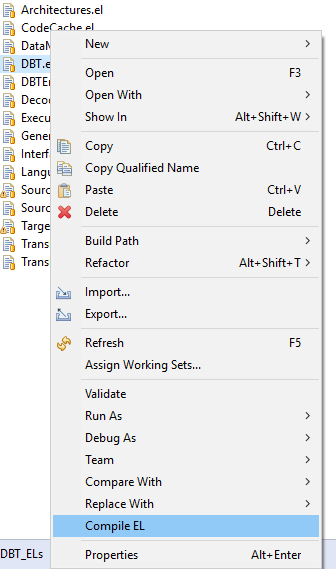
\includegraphics[width=0.4\linewidth]{Images/compileEL}
		\caption{Compile EL scripts}
		\label{fig:compileel}
	\end{figure}
	
	This will generate a series of files Java and XML. The two most important directories are the \texttt{Configs} where the configurable XML is stored and the \texttt{SpecificElaborations} where it generates a template for each component. 
	If the template change is not desired, and because when the EL is compiled the file is overwritten, the XML of a specific component should be altered to have the specific elaboration file that is wanted.
	In the case of the \texttt{Generator} it is wanted the \texttt{SpecificGeneratorElaborator} instead of template that is set by default so the XML is altered as shown in the line  of the following XML.
	\begin{EL}
	<component type="Generator">
		<elaboration default="SpecificGeneratorElaboratorTemplate">SpecificGeneratorElaborator</elaboration>
			<properties>
				<property type="bool" name="optimizations" default="false"><value>
					<element>true</element>
				</value>
			</property>
		</properties>
	</component>
	\end{EL}
	
	The source files of DBT with annotations should be placed in the same folder of the specific elaboration for the component that models that code, or in the folder shared sources if the source as annotations that refer to different components. 
	
	The annotations that the elaborator for the generator replaced are described in table \ref{annotationTable}.
	\begin{table}[h]
		\caption{Code generation functions.}
		\label{annotationTable}
		\centering
		\begin{tabular}{|l||l||l|}
			\hline
			\textbf{Annotations} 	& \textbf{File} 			& \textbf{Type}\\ \hline
			Generator\_optimization & TargetArch\_CortexM3.h 	& Property replacement \\ \hline
			Generator\_cacheCode	& TargetArch\_CortexM3.cpp	& Interface Functions replacement \\ \hline
			Generator\_getPC		& TargetArch\_CortexM3.cpp	& Interface Functions replacement \\ \hline
			Generator\_readDataMem	& TargetArch\_CortexM3.cpp	& Interface Functions replacement \\ \hline
			Generator\_eoBB			& TargetArch\_CortexM3.cpp	& Interface Functions replacement \\ \hline
			Generator\_eoExec		& TargetArch\_CortexM3.cpp	& Interface Functions replacement \\ \hline
			Generator\_tracing		& SharedSources/types.h		& String replacement \\ \hline
			
		\end{tabular}
	\end{table}	
	
	The table shows that the generator is only going to alter the files TargetArch\_CortexM3.h and TargetArch\_CortexM3.cpp and a shared source named types.
	
	The third column of the table as the type of replacement. As it is possible to observe there are three types the first one is replace the annotation with the value of a property that is altered in the XML file. 
	
	The second type is the interface functions replacement to respect the interfaces from the model. If a component makes reference to a service in component, the user needs to alter the code and replace a annotation, that is according with the function of that interface, in order to respect the reference architecture. 
	
	And last type is a direct string replacement. In this case it is used a property to know if the elaborator should comment or simply delete the annotation. The elaborator replace with a string with the comment or with nothing, deleting the annotation from the source file.
	
	The process to make the specific elaborator for a component, is to use the AbstractElaborator API to open sources and replace their annotations.
	
	\begin{lstlisting}[language=Java]
	package EL.SpecificElaborations.Generator.SpecificGeneratorElaborator;  
	
	import EL.Components._Generator;
	import EL.Elaborations.AbstractGeneratorElaborator;
	import EL.ElaborationError;
	import java.util.ArrayList;
	import EL.ConfigReader.SpecificConfigReader;
	import EL.Elaborations.*;
	import EL.ConfigReader.*;
	import EL.Components.*;
	
	public class SpecificGeneratorElaborator extends AbstractGeneratorElaborator {
	SpecificConfigReader scr = null;
	
	public void generate(){
	System.out.println("This is the Generator template specific elaboration.");
	openAnnotatedSource("TargetArch_CortexM3.h");
	replaceAnotation("Generator_optimization",String.valueOf(target.get_optimizations()));
	
	openAnnotatedSource("TargetArch_CortexM3.cpp");		
	AbstractTranslationCacheElaborator TCacheElab = (AbstractTranslationCacheElaborator) getElaborator((_TranslationCache) target.get_r_TCache());
	replaceAnotation("Generator_cacheCode", (String) TCacheElab.getI_TCacheElaboratorCacheCode());
	
	AbstractSourceEnvElaborator SrcEnvElab = (AbstractSourceEnvElaborator) getElaborator((_SourceEnv) target.get_r_SrcEnv());
	replaceAnotation("Generator_getPC", (String) SrcEnvElab.getI_SrcEnvElaboratorGetPC());
	
	AbstractDataMemoryElaborator DataMemElab = (AbstractDataMemoryElaborator) getElaborator((_DataMemory) target.get_r_DMem());
	replaceAnotation("Generator_readDataMem", (String) DataMemElab.getI_DMemElaboratorReadDataMem());
	
	AbstractDBTEngineElaborator DBTEngineElab = (AbstractDBTEngineElaborator) getElaborator((_DBTEngine) target.get_r_EngineState());		
	
	replaceAnotation("Generator_eoBB", (String) DBTEngineElab.getI_EngineStateElaboratorEoBB());
	replaceAnotation("Generator_eoExec", (String) DBTEngineElab.getI_EngineStateElaboratorEoExec());
	
	openAnnotatedSharedSource("types.h");
	if(target.get_trgCodeTracing()==false)
	replaceAnotation("Generator_tracing","//");
	else
	replaceAnotation("Generator_tracing","");
	}
	\end{lstlisting}
	
	After the specific elaboration file is completed with the strings that should substitute the annotations, it is possible to build the final sources that will be stored into the directory FinalFiles. To do that, the commands presented in the next figures should be executed.
	
	The first one (Figure \ref{fig:build}) generates the \texttt{.class} files for each component, abstract elaboration, specific elaboration and so on. And after that generates the Elaborator from that files.
	
	The second one (Figure \ref{fig:runElaborator} runs the Elaborator that will generate the final sources files by replacing the annotations and copy the files to the FinalFiles folder. It executes all the code of the specific elaboration, and can open the XML files to get a property value. At the end if everything is fine and the sources were generated it prints the message: "All final files successfully generated!". If something goes wrong in the elaboration, if it has some kind of error in the elaboration files it prints a error message informing the user.
	
	\begin{figure} [H]
		\centering
		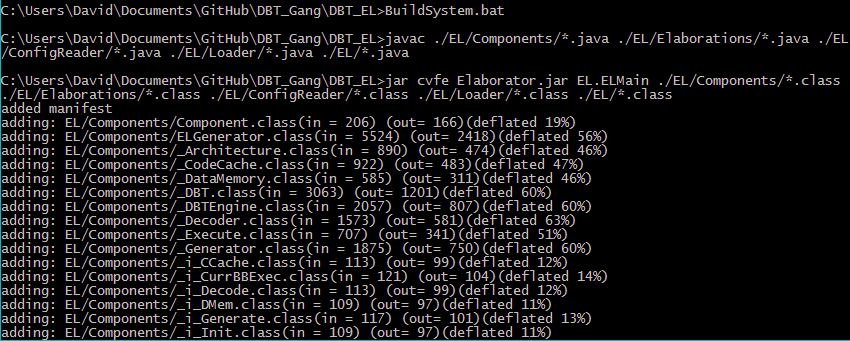
\includegraphics[width=1\linewidth]{Images/script}
		\caption{Generation of the elaborator.}
		\label{fig:build}
	\end{figure}
	
	\begin{figure} [H]
		\centering
		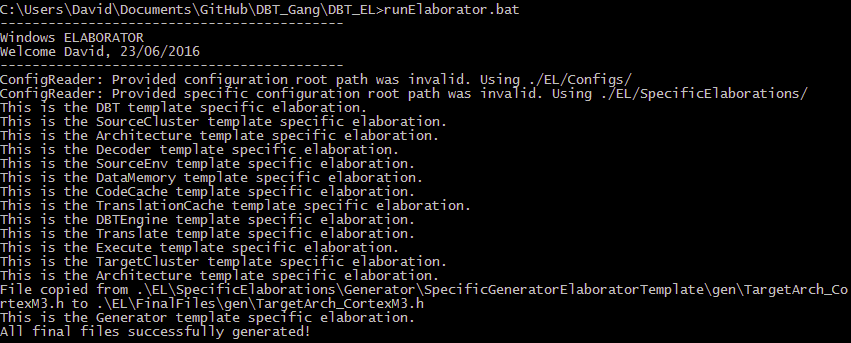
\includegraphics[width=1\linewidth]{Images/scriptRunElaborator}
		\caption{Running the elaborator.}
		\label{fig:runElaborator}
	\end{figure}
	
	The final files will have all the notations replaced with the String that the user defined. For example, the annotation in the figure \ref{fig:annotation}, it will be replaced by the property optimizations. 
	
	\begin{figure} [H]
		\centering
		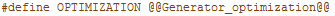
\includegraphics[width=0.5\linewidth]{Images/anotation.PNG}
		\caption{Annotation of optimizations.}
		\label{fig:annotation}
	\end{figure}
	
	The annotation will be replaced with the value that the user put in the XML. If it has default value and the user didn't set other value in the XML it will be replaced by the default value as is shown in the figure \ref{fig:annotationReplaced}.
	
	\begin{figure} [H]
		\centering
		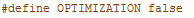
\includegraphics[width=0.3\linewidth]{Images/anotationReplaced.PNG}
		\caption{Annotation replaced by it's default value.}
		\label{fig:annotationReplaced}
	\end{figure}
	
	\section{Optimizations}
	
	\par When the group finished the main objective of this project, it was decided to contribute in some way to the algorithm. Over this report there were some references to optimizations, but it was not implemented in the assigned code. 
	\par When studying how the code was generated for the target architecture, that was detected the occurrence of irrelevant load instructions. The situation is easily understandable in the next example that shows the translated code for the source instruction \texttt{INC DPTR}.
	\begin{ARM}
	;R4 is the memory base and to it is added an offset
	
	;Load of the contents of (R4,#82) to R5.	
	LDRH R5,[R4,#82]
	;Incremenent the value of R5.
	ADDW R5, R5, #1
	;Store the value of R5 in (R4 + #0x82) position
	STRH R5, [R4 + #0x82]
	;Load the value of (R4, #0x82) to R5
	LDRB R5,[R4,#0x82]
	\end{ARM}
	
	\par The Load is not necessary in this situation because the value of R5 did not change between instructions. To save some cycles, it was introduced on simple algorithm to the load and store operations.
	\par When a store instruction occurs, the value of the PC is stored into a auxiliar variable \texttt{auxPC\_Source}. The information about the register being used to store and the memory position are also stored into the variables \texttt{Optim\_DReg} and \texttt{auxR5} respectively. 
	\begin{Cpp}
	#if OPTIMIZATION == true
		auxPC_source = env->PC;
		Optim_DReg = SReg;
		auxR5 = imm; 
	#endif
	\end{Cpp}
	\par When a load instruction occurs, the register is compared with the value of \texttt{Optim\_DReg} and the immediate with the value stored in \texttt{auxR5}. Then, if the condition is true, it is verified if the actual PC is not more than three positions forward. This condition is necessary due to the variable size of the source architecture instructions' size. 
	\par If this condition is true, then the value of \texttt{auxR5} is cleaned and the function ends here. There is no need to load from memory because the value of the register is valid.
		
	\begin{Cpp}
	#if OPTIMIZATION == true
	if (DReg == Optim_DReg && auxR5 == imm){
		if (auxPC_source == ((env->getPC)-1) || auxPC_source == ((env->PC)-2) || auxPC_source == ((env->PC)-3)){
			auxR5 |= 0xffff;
			return;
		}
	}
	#endif 
	\end{Cpp}
	
	\par With this simple algorithm, the number of cycles is reduced in more than 1.45\% when compared to the number of cycles executed when the optimizations are turned off. The group made various tests to the algorithm to conclude that it was the best approach. Table \ref{tab:opt} shows the different results.
	
	\begin{table}[H]
		\centering
		\caption{Optimizations results.}
		\label{tab:opt}
		\begin{tabular}{l|lll}
			\hline
			\textbf{Description} & \begin{tabular}[c]{@{}l@{}}\textbf{Number} \\ \textbf{of cycles}\end{tabular} & \begin{tabular}[c]{@{}l@{}}\textbf{Exit} \\ \textbf{address}\end{tabular} & \begin{tabular}[c]{@{}l@{}}\textbf{Percentual} \\ \textbf{optimization}\end{tabular} \\ \hline
			Without optimization & 11393410026 & 0x88f & 0\% \\
			\begin{tabular}[c]{@{}l@{}}With the first optimization \\ approach\end{tabular} & 11381943769 & 0x88f & 0,1006393781\% \\
			\begin{tabular}[c]{@{}l@{}}Removing one 'if' condition\\ in store instructions \\ (first approach)\end{tabular} & 11228165032 & 0x88f & 1,450355895\% \\
			\begin{tabular}[c]{@{}l@{}}Changing the 'if' order in load \\ instruction\end{tabular} & 11471817519 & 0x88f & -0,6881828427\% \\
			\begin{tabular}[c]{@{}l@{}}Removing the condition \\ 'auxPC\_source == ((env-\textgreater PC)-3)' \\ in the second 'if'\end{tabular} & 11246271258 & 0x88f & 1,291437486\% \\
			\hline
		\end{tabular}
	\end{table}

	
	\section{Results}
	
	The implementations should be tested in order to validate if they are working properly.
	To do that we will compare files with what it should generate and observe if the elaborator is working properly. The tests that will be done are explain in detail in the chapther Test Plans.
	
	\paragraph{Single Elaboration Test}
	This test is to validate the overall process, it was created a dummy component with the language C and the following annotation. 
	
	\begin{EL}
		compile dummy
		component dummy(C){}
		language C {annotation: "@"}
	\end{EL}
	
	
	It was created a file with just a annotation and put in the same folder of the specific elaboration. The annotation was named DBT.Then it was add in the elaborator the following functions:
	
	\begin{lstlisting}[language=Java]
		openAnnotatedSource("file.c");
		replaceAnotation("DBT","it works");
	\end{lstlisting}
	
	The result was that the file was copy to \texttt{FinalFiles} folder with annotation replaced by the string "it works".
	
	\paragraph{Integration Test}
	The next test is to make all the specific elaborations and place the annotated source code in the right place, and verify if with all the elaborations build. With this test we verify that all annotation with properties change to the default value of that property, all the files were generated, all the annotations were replaced and that the shared sources were replaced in right place by the right component.
	
	\paragraph{Properties Test}
	In this test we alter the properties of the XML and watch them change by replacing the annotation with the property value. This test work just as was described.
		
	\paragraph{Execution Test}
	In the final test, the generated final files that were generated previously and created a project in IAR Workbench. The files were compiled with zero errors. The results of the execution of that code are shown in the following code and validate this test.
	
	\begin{lstlisting}
	MicroSemi SmartFusion2
	Device running on   
	M2S150        
	
	TBuffer starts at 0x20005318, with a size of 8192 bytes
	Buffer end address is 0x20007318
	cache size 0 NOT BEING USED. CODE BUFFER IN USE
	XDATA_SIZE base address is 0x20007320
	end address is 0x20009320
	Source program at 0x60040000 address, with size of 32768 bytes
	Exit address at 0x34f7
	Entering envReset()
	
	Varable env.dataMem at 30000000

	Varable env.dataMem[SP] at 30000081
	
	Entering condCodedHandlerInit()
	(int *)(env.dataMem) = 0x30000000
	(int*)&env.dataMem[PSW] = 0x300000d0
	Configuring Sniffer module...
	Enabling BusFault...
	Configuring sniff address as READ_EN...
	Enabling Sniffer Module...
	Checking Sniffer config:
	sniffer_ctrl: 1
	sniffer_watch_address: 0x300000d0
	sniff_en: 2
	codeCache.load()
	Starting runDBT now...
	
	...trans 0x0
	## 0x0 MISS ##
	PUSH {R4, R5, R6, R7, R8, R9, LR, }
	MOV R4, R0
	# 0x0 <=> 0x2000531e
	MOVW R9,#102
	MOVW R8,#20696
	MOVT R8,#8192
	STRH R9,[R8, #0]
		LJMP 0x0066
	
	POP {R4, R5, R6, R7, R8, R9, PC, }
	exec...

	\end{lstlisting}
	After all these tests results, it is possible to verify that all the things are working fine and that the code that is generated is fully functional and can be used to binary translation.
	
	
	
	
%END CONCEPTION CHAPTER
%-------------------------------------------
%START CONCLUSION CHAPTER

\chapter{Conclusion}

	\par This project was divided in three phases: analysis, design and implementation. In the analysis, it was made a deep study about modeling, which contemplate the Service Component Architecture and Domain Specify Languages. The Elaboration Language and the details that are needed for the user and the designer were covered. The analysis chapter ends with the study of the Dynamic Binary Translator: its source and target architectures and the architectural model.
	\par During the Design Chapter, the focus was on the code interpretation. A deeper study was made around the code analysis and the code refactor. The code generation also takes an important role because is the main focus of the group. The reference architecture model is presented with all the components and interfaces. The chapter ends with the tests' plans.
	\par The implementation shows the concretization of the project. The model was translated to Elaboration Language and the respective Elaborations were made. The Optimizations section was an extra work that the group decided to do to contribute to the code in some way. After this, the results are exposed.
	\par All the project objectives were complete and the group is satisfied with the results. Modeling an dynamic binary translator was very interesting because the group learned about two new concepts and acquire competences to solve future problems. 

%END CONCLUSION CHAPTER
%-------------------------------------------
\newpage
	
\bibliography{mybib}{}
%\bibliographystyle{ieeetr}
	
\end{document}
